% ----------------------- TODO ---------------------------
% Change per hand-in
\newcommand{\NUMBER}{1} % exercise set number
\newcommand{\EXERCISES}{5} % number of exercises

\newcommand{\COURSECODE}{ }
\newcommand{\TITLE}{Optical Microscope}
\newcommand{\STUDENTA}{CBL Sample preparation}
\newcommand{\DEADLINE}{DEADLINE}
\newcommand{\COURSENAME}{ }
% ----------------------- TODO ---------------------------

\documentclass[a4paper]{scrartcl}

% \usepackage[utf8]{inputenc}
\usepackage[british]{babel}
\usepackage{amsmath}
\usepackage{amssymb}
\usepackage{fancyhdr}
\usepackage{color}
\usepackage{graphicx}
\usepackage{lastpage}
\usepackage{listings}
\usepackage{tikz}
\usepackage{pdflscape}
\usepackage{subfigure}
\usepackage{float}
\usepackage{polynom}
\usepackage{hyperref}
\usepackage{tabularx}
\usepackage{forloop}
\usepackage{geometry}
\usepackage{listings}
\usepackage{fancybox}
\usepackage{tikz}
\usepackage{siunitx}
\usepackage{mathtools}
\usepackage{fontspec}
\usepackage{soul}

\newcommand*\Let[2]{\State #1 $\gets$ #2}

% Matrix notation
\newcommand{\matr}[1]{\mathbf{#1}}

% Custom units
\DeclareSIUnit\bar{bar}

% Margins
\geometry{a4paper,left=3cm, right=3cm, top=3cm, bottom=3cm}

% Colours
\definecolor{warning}{HTML}{DA073B}

% Header and footer setup
\pagestyle {fancy}
\fancyhead[L]{\TITLE}
\fancyhead[C]{\STUDENTA}
\fancyhead[R]{\today}

\fancyfoot[L]{\COURSECODE}
\fancyfoot[C]{\COURSENAME}
\fancyfoot[R]{Page \thepage /\pageref*{LastPage}}

\setmainfont{Inter}

\begin{document}

\section*{Microscopy}
\begin{figure}[h]
	\begin{center}
		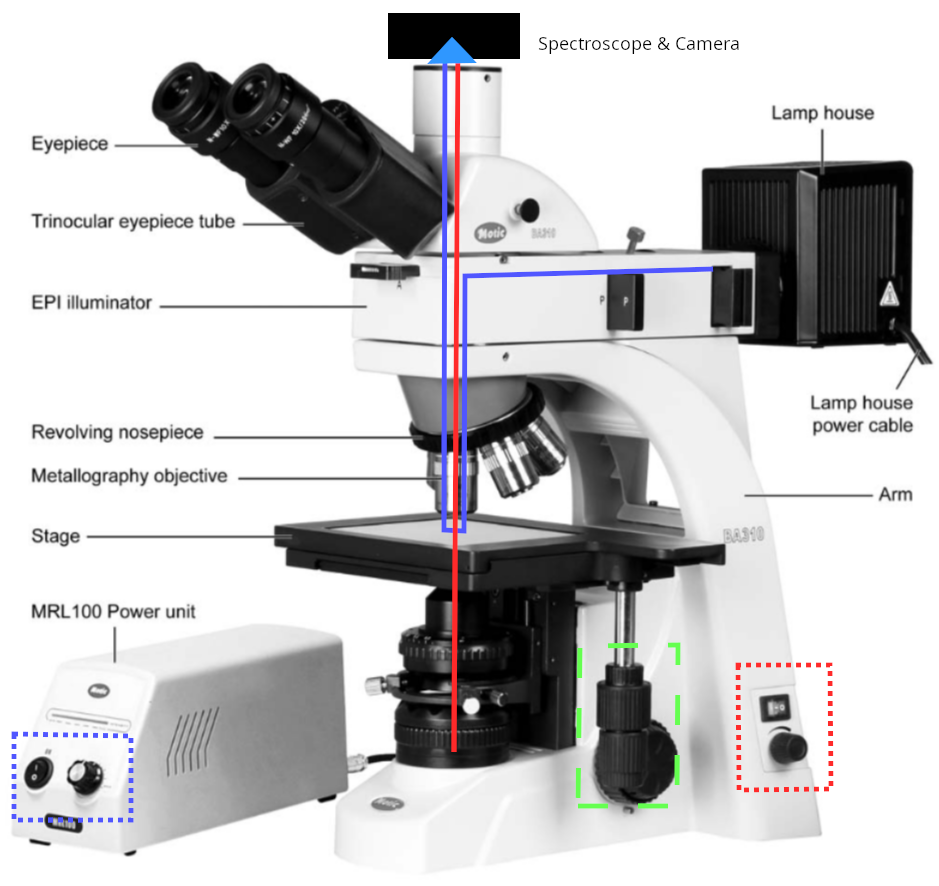
\includegraphics[width=.6\textwidth, keepaspectratio]{figures/illum_paths.png}
	\end{center}
	\caption{Overview of the relevant parts of the microscope. The transmittance and reflectance microscopy light paths and their respective luminance controls are indicated by the red and blue lines and dotted boxes respectively. The `x`, `y` and `z` stage control are denoted by the green dashed box. The stage `x` and `y` control are on the stem extending down from the platform and the `z` or rough focus control is the big knob on the side of the microscope body. Another rough focus as well as fine focus adjustment is mirrored on the other side of the microscope body.}
	\label{fig:illum_paths}
\end{figure}

\subsection*{Sample Inspection}
\begin{enumerate}
	\item For cleanliness, prepare your sample on a glass microscope slide, these can be found in the drawers. Select the smallest magnifying objective on the revolving nosepiece and move the stage all the way down with the focus knob.\\
		Place the glass slide with the sample on the stage.
	\item Turn on the light bulb for the illumination mode you want to use. For transparent samples you can use both transmission or reflectance microscopy, for opaque samples you can only use reflectance. The switches and luminance controls are denoted by the blue and red dotted boxes in Figure~\ref{fig:illum_paths}.
	\item Whilst looking through the eyepieces adjust focus until a sharp image appears. To better pinpoint where you are looking you can close the respective aperture of the illumination mode you are using to create a small bright spot on your sample and move the stage to the desired location.
	\item To magnify your image further you can revolve the next larger magnifying objective into the optical path by rotating the revolving nosepiece clockwise until it `clicks` into position. Refocus using the fine focus knob. Repeat until the desired magnification is reached.\\
		\colorbox{warning!30}{\parbox{\linewidth}{Watch out for crashes with the larger magnifying objectives!}}
	\item When you are done using the microscope switch to the smallest magnifying objective by rotating the revolving nosepiece counter-clockwise. Lower the stage fully and turn off all the lights.
\end{enumerate}

\subsection*{Using the Camera}
\begin{enumerate}
	\item Log-in on the computer to the left of the microscope with the username and password on the screen. Launch the Moticam software through the shortcut on the desktop. In the toolbar on the left-hand side of the main screen click the button called `live view`, this will open up a new window with a live preview of the camera.
	\item Readjust fine focus such that the image on the camera is sharp as the focus is slightly mismatched with respect to the eyepieces.
	\item On the right-hand side of the live view there are a series of buttons that will open up options for annotations, exposure and colorbalance; adjust these to your liking.
	\item At the top of the screen select the correct calibration for your magnifying objective.
	\item Take an image by opening up the camera controls on the right-hand side of the `live view` window. Use the HDR option if you which to perform any operations on the final image. The higher bit depth will make i.e. edge detection algorithms more robust.
\end{enumerate}

\section*{Spectroscopy}
\begin{figure}[h]
\begin{center}
	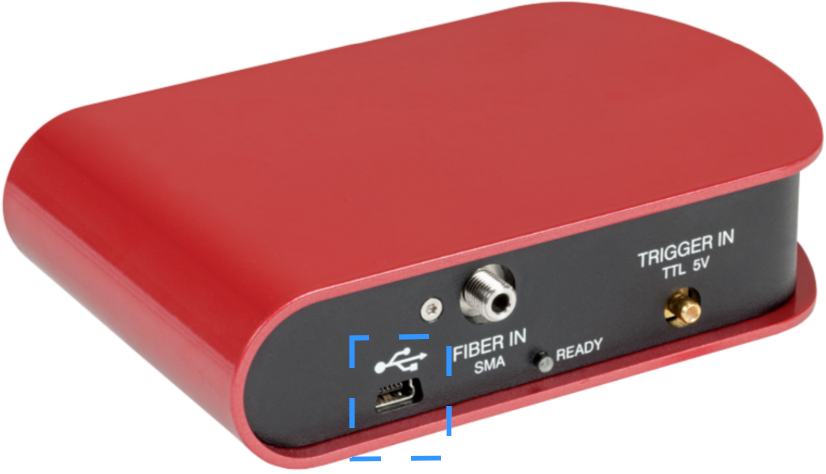
\includegraphics[width=0.5\textwidth, keepaspectratio]{figures/spectroscope.png}
\end{center}
\caption{Overview of the spectroscope. Highlighted is the socket where the USB-cable needs to be plugged in before use and unplugged after use.}
\label{fig:spectroscope}
\end{figure}
\subsection*{Software start-up}
\begin{enumerate}
	\item Log into the computer with the username and password on the screen. On the desktop click the shortcut `ThorSpectra` to start up the spectroscope's software package.
	\item Plug the USB-cable into the spectroscope.
	\item In the spectroscope software screen click the `Instrument` button in the header, then click the `Connect Devices` button in the toolbar above the plotting window
	\item With the microscope's lights off press the button `Single` to acquire a single spectrum. If the device was successfully connected a spectrum should appear.
\end{enumerate}

\subsubsection*{Aiming the optical fibre}
\begin{minipage}[t]{.58\linewidth}
	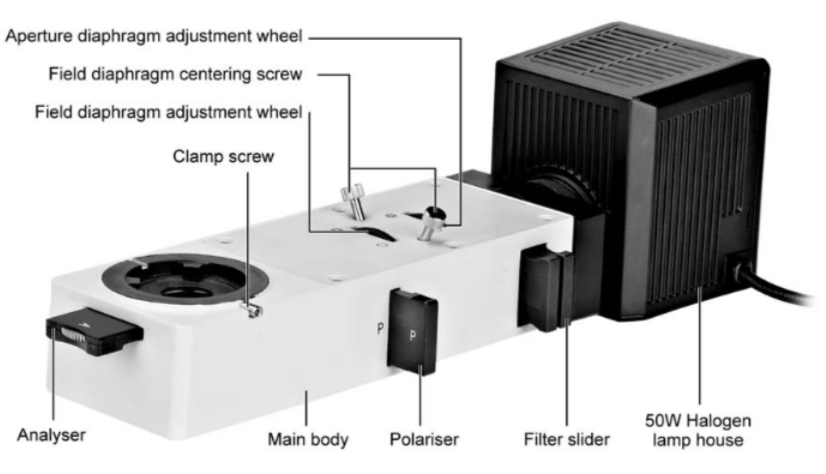
\includegraphics[width=1\linewidth, keepaspectratio]{figures/epi_aper.png}
	\captionof{figure}{Overview of the EPI-illumination system of the microscope. The apertures and filters in this system will be used for the micro-reflectance spectroscopy experiment and for aligning the fibre.}
	\label{fig:fibre}
\end{minipage}\hspace{0.04\linewidth}%
\begin{minipage}[t]{.38\linewidth}
	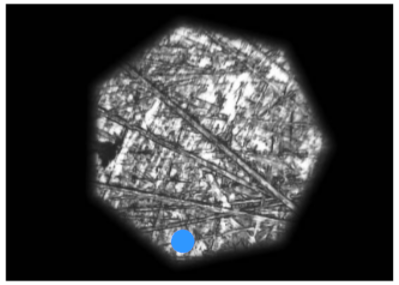
\includegraphics[width=1\linewidth, keepaspectratio]{figures/fiber_align.png}
	\captionof{figure}{Example photograph a taken with the field diaphragm fully closed. Highlighted with the blue dot is the rough position of the optical fibre.}
	\label{fig:apertures}
\end{minipage}

\begin{enumerate}
	\item Aiming the optical fibre starts by finding your sample and bringing it to the proper focus.
	\item Turn on the EPI-illumination or reflectance illumination bulb by adjusting the controls highlighted with blue in Figure~\ref{fig:illum_paths}.
	\item Fully close the EPI-illumination field diaphragm by adjusting the slider at the top of the microscope body. For reference of the proper slider see Figure~\ref{fig:apertures}.
	\item Aim the fibre by placing the imaginary blue dot over the sample region you want to acquire a spectrum from by adjusting the stage position.
	\item Adjust focus such that the outline of the diaphragm is as sharp as possible.
\end{enumerate}

\subsubsection*{Micro-reflectance spectroscopy}
\begin{enumerate}
	\item Start by tuning the exposure settings of spectroscope. Determine which is brighter, your sample or your substrate. Tune the exposure on the brighter surface. The exposure time can be set when pressing the button labelled `instrument` in the header followed by entering a number on the right side of the lowest toolbar and pressing enter. The maximum intensity should be close to `1` for high signal-to-noise ratio. For maximum brightness in EPI-illumination mode the exposure time should be roughly \SI{400}{\milli \second}. To acquire a single test spectrum press `CTRL + N` whilst shaking the fibre. Continue changing the exposure until you have maximised the intensity without over saturating the spectroscope.
	\item Press the `A` trace button in the plotting window. Then press `ALT - A` or right-click the `A` trace button and press averaging to open the averaging window. Set the amount of spectra and click `set to fixed when finished`. You can now acquire the set amount of spectra by shaking the fibre and pressing `CTRL-R` or clicking `Repeat`.
	\item Acquire an amount of spectra of your substrate in the `A` trace and an amount of spectra of your sample in the `B` trace.
	\item To calculate the differential reflectance we need to compute $(R-R_0)/R$ where $R$ is the sample and $R_0$ the substrate. Computing this quantity is done by right-clicking trace `C` and selecting `Compute` → `User Defined` and filling in the formula `(B-A)/B` and pressing `Compute`.
	\item Trace `C` will now display the computed micro-reflectance spectrum. To improve the view right-click `C` and press `move to secondary axis`. You can now click the y-label on the right of the plot to change the limits. Change these limits to $0\%$ for the lower limit and $170\%$ for the upper limit. Adjust if needed.
	\item To better read out the peak position you can click in the header `Marker`, then the `Marker 1` button or press `CTRL+1`. You can now move the marker and read out the value of its position in the pop-up.
	\item For more advanced software features look at the `User Guide` on Teams or ask for help on options like smoothing, peak detection and exporting data.\\
		Some other useful tips are included at the end of this document in the Tips section.
\end{enumerate}
\newpage

\subsubsection*{Micro-transmittance spectroscopy}
\begin{figure}[h]
\begin{center}
	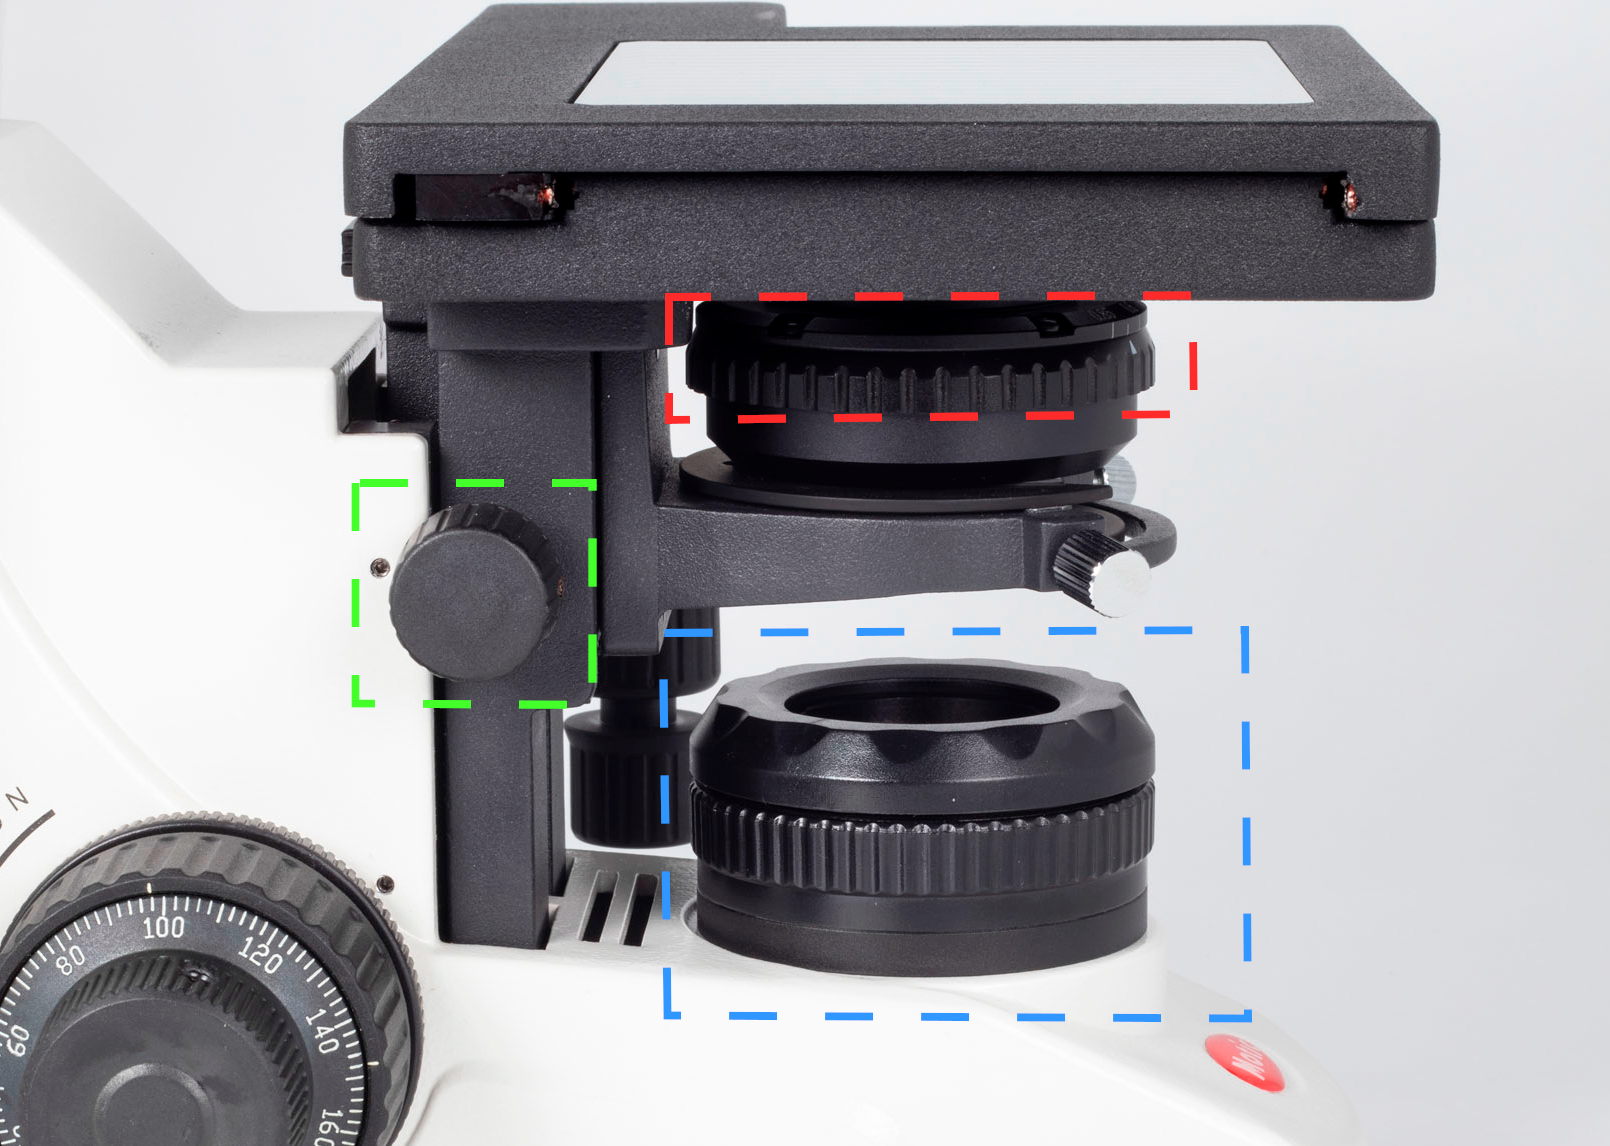
\includegraphics[width=0.5\linewidth, keepaspectratio]{figures/kohler.png}
\end{center}
\caption{Overview of the left-hand side of the microscope body and stage assembly. Highlighted are the controls of interest for micro-transmittance spectroscopy, namely: in the blue dashed box is the field diaphragm for the transmission illumination; in the red dashed box is the field aperture; and; in the green dashed box is the objective condenser focus.}
\label{fig:kohler}
\end{figure}

\begin{enumerate}
	\item Micro-transmittance works roughly the same as carrying out micro-reflectance. Outlined below are a few important differences.
	\item Exposure adjustment should probably be done on the transparent substrate as this is most likely the brighter part of the sample.
	\item Set up the microscope for Köhler illumination. To achieve this fully close the transmission field diaphragm by rotating the ring below the lower light opening (blue box Figure~\ref{fig:kohler}) and adjust the condenser position with the knob in the green dashed box such that the diaphragm edges are sharp and in focus.
	\item To calculate the transmittance spectrum we need to compute $R/R_0$ where $R$ is the sample and $R_0$ the substrate. Computing this quantity is done by right-clicking trace `C` and selecting `Compute` → `User Defined` and filling in the formula `B/A` and pressing `Compute`.
\end{enumerate}


\end{document}

